%%%%%%%%%%%%%%%%%%%%%%%%%%%%%%%%%%%%%%%%%
% Beamer Presentation
% LaTeX Template
% Version 1.0 (10/11/12)
%
% This template has been downloaded from:
% http://www.LaTeXTemplates.com
%
% License:
% CC BY-NC-SA 3.0 (http://creativecommons.org/licenses/by-nc-sa/3.0/)
%
%%%%%%%%%%%%%%%%%%%%%%%%%%%%%%%%%%%%%%%%%

%----------------------------------------------------------------------------------------
%	PACKAGES AND THEMES
%----------------------------------------------------------------------------------------

\documentclass{beamer}

\mode<presentation> {

% The Beamer class comes with a number of default slide themes
% which change the colors and layouts of slides. Below this is a list
% of all the themes, uncomment each in turn to see what they look like.

%\usetheme{default}
%\usetheme{AnnArbor}
%\usetheme{Antibes}
%\usetheme{Bergen}
%\usetheme{Berkeley}
%\usetheme{Berlin}
%\usetheme{Boadilla}
%\usetheme{CambridgeUS}
%\usetheme{Copenhagen}
%\usetheme{Darmstadt}
%\usetheme{Dresden}
%\usetheme{Frankfurt}
%\usetheme{Goettingen}
%\usetheme{Hannover}
%\usetheme{Ilmenau}
%\usetheme{JuanLesPins}
%\usetheme{Luebeck}
\usetheme{Madrid}
%\usetheme{Malmoe}
%\usetheme{Marburg}
%\usetheme{Montpellier}
%\usetheme{PaloAlto}
%\usetheme{Pittsburgh}
%\usetheme{Rochester}
%\usetheme{Singapore}
%\usetheme{Szeged}
%\usetheme{Warsaw}

% As well as themes, the Beamer class has a number of color themes
% for any slide theme. Uncomment each of these in turn to see how it
% changes the colors of your current slide theme.

%\usecolortheme{albatross}
%\usecolortheme{beaver}
%\usecolortheme{beetle}
%\usecolortheme{crane}
%\usecolortheme{dolphin}
%\usecolortheme{dove}
%\usecolortheme{fly}
%\usecolortheme{lily}
%\usecolortheme{orchid}
%\usecolortheme{rose}
%\usecolortheme{seagull}
%\usecolortheme{seahorse}
%\usecolortheme{whale}
%\usecolortheme{wolverine}

\usefonttheme{serif} 

%\setbeamertemplate{footline} % To remove the footer line in all slides uncomment this line
%\setbeamertemplate{footline}[page number] % To replace the footer line in all slides with a simple slide count uncomment this line

\setbeamertemplate{navigation symbols}{} % To remove the navigation symbols from the bottom of all slides uncomment this line
}

\usepackage{graphicx} % Allows including images
\usepackage{booktabs} % Allows the use of \toprule, \midrule and \bottomrule in tables
\usepackage[T1]{fontenc}
\usepackage[utf8]{inputenc}
\usepackage{amsmath}
\usepackage{color}
\usepackage[czech]{babel}
\usepackage{lmodern}  
\usepackage{rotating}
\usepackage{scrextend}
\usepackage{pifont}
\usepackage{hyperref}
\usepackage{bm}

%----------------------------------------------------------------------------------------
%	TITLE PAGE
%----------------------------------------------------------------------------------------

\title[Týden x]{Praktikum z ekonometrie - Týden x} % The short title appears at the bottom of every slide, the full title is only on the title page

\author{VŠE Praha} % Your name
\institute[4EK417] % Your institution as it will appear on the bottom of every slide, may be shorthand to save space
{
% Your institution for the title page
\medskip
\textit{Tomáš Formánek} % Your email address
}
\date{} % Date, can be changed to a custom date

\begin{document}

\begin{frame}
\titlepage % Print the title page as the first slide
\end{frame}

\begin{frame}
\frametitle{Obsah} % Table of contents slide, comment this block out to remove it
\tableofcontents % Throughout your presentation, if you choose to use \section{} and \subsection{} commands, these will automatically be printed on this slide as an overview of your presentation
\end{frame}

%----------------------------------------------------------------------------------------
%	PRESENTATION SLIDES
%---------------------------------------------------------------------
\section{Úvod}
\begin{frame}{Úvod}


\end{frame}
%---------------------------------------------------------------------
\section{Prostorová autokorelace}
\begin{frame}{Prostorová autokorelace}
\begin{figure}
	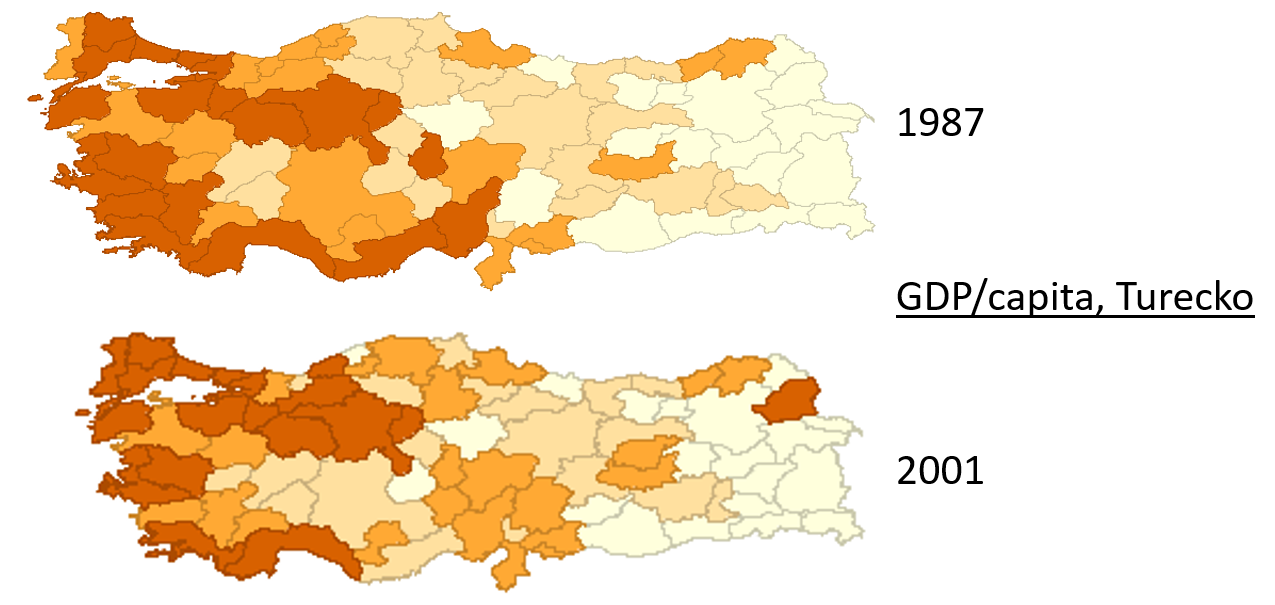
\includegraphics[width=.9\textwidth]{IMG/sp_auto1.PNG}
\end{figure}
\end{frame}
%---------------------------------------------------------------------
\begin{frame}{Prostorová autokorelace}
\begin{figure}
	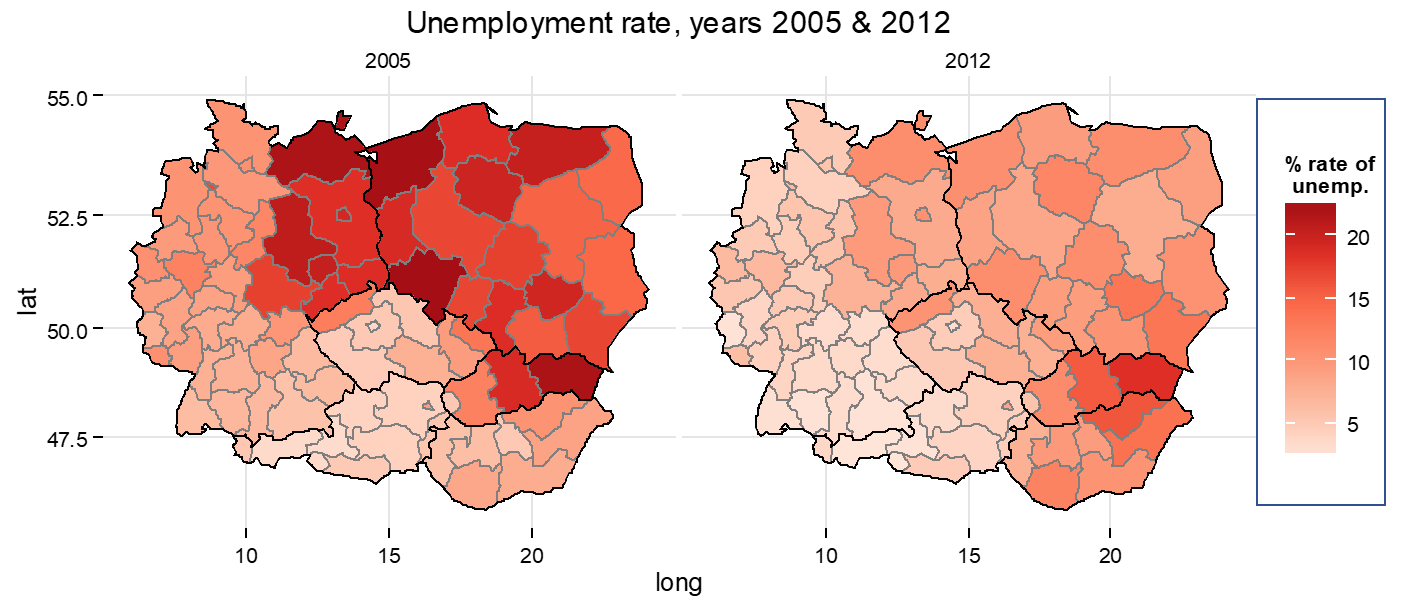
\includegraphics[width=.9\textwidth]{IMG/sp_auto2.PNG}
\end{figure}
\end{frame}
%---------------------------------------------------------------------
\begin{frame}{Prostorová autokorelace}
\begin{itemize}
\item Prostorové modely umožňují rozlišit vliv geografických faktorů (prostorová autokorelace, spill-over efekty) od působení dalších relevantních proměnných, které mohou být např. ovlivněny nástroji makroekonomické politiky.
\item Pozorování (prostorové jednotky) jsou charakterizovány geografickou polohou (geo-coded), sledujeme vzdálenosti mezi jednotkami.
\end{itemize}
\end{frame}
%---------------------------------------------------------------------
\begin{frame}{Prostorová autokorelace}
\textbf{Prostorová závislost/autokorelace – příklady}
\begin{itemize}
	\item Ceny nemovitostí závisejí na užitných vlastnostech (byt: m$^2$, počet místností, výtah, $\dots$) ale i na lokalitě. Ceny v dané lokalitě vykazují určitou míru podobnosti$\dots$ Obvykle zde platí kladná prostorová autokorelace. 
	\item Tržby benzínových pump na dálnicích závisejí na vzdálenosti od aglomerace (resp. na hustotě provozu, která se vzdáleností od aglomerace slábne). Speciální případ jednorozměrné prostorové závislosti (obvykle uvažujeme 2D vzdálenosti a závislosti).
	\item Zvýšená policejní přítomnost/aktivita v určité oblasti (okrese) sníží míru kriminality, ale může způsobit přesun nelegálních aktivit do okolních oblastí (negativní autokorelace).
	\item Makroekonomické šoky (pozitivní i negativní) se mohou "přelévat" mezi ekonomikami. 
\end{itemize}
\end{frame}
%---------------------------------------------------------------------
\begin{frame}{Prostorová autokorelace}
\begin{itemize}
	\item \textit{"Prostorová závislost popisuje vztah pozorovaného atributu (hodnota sledované proměnné) v určité oblasti vůči pozorovaným atributům v okolních oblastech."} (Fotheringham et al, 2002).
	
	\item \textit{"Prostorová autokorelace ($\dots$) je korelace mezi pozorovanými hodnotami jedné proměnné, již lze přisoudit výhradně geografické blízkosti jednotlivých pozorování ($\dots$)."} (Griffith, 2003).
\end{itemize}
\end{frame}
%---------------------------------------------------------------------
\begin{frame}{Prostorová autokorelace}
\textbf{Prostorová závislost – diskuse}
\begin{itemize}
	\item Velká část prostorových efektů (prostorové závislosti) úzce souvisí s vynechanými faktory (důležité vysvětlující proměnné modelu).
	
	\item Prostorová autokorelace - proxy proměnná pro řadu nepozorovatelných nebo obtížně kvantifikovatelných faktorů. Například, jde-li o trh práce (nezaměstnanost) v EU: 
	\begin{itemize}
		\item Dojíždění za prací mezi okresy/kraji/státy, resp. konzistentní měření tohoto jevu.
		\item Jazykové, kvalifikační, administrativní bariéry na pracovním trhu.
		\item Vzdušné vzdálenosti vs. toplogie vs. kvalita a hustota dopravní sítě. 
	\end{itemize}
	\item Prostorové modely mohou poskytnout dobře interpretovatelný a prakticky využitelný způsob analýzy makroekonomické (regionální) dynamiky.
\end{itemize}
\end{frame}
%---------------------------------------------------------------------
\section{Definice sousedících oblastí (Neighbours)}
\begin{frame}{Definice sousedících oblastí (Neighbours)}
\begin{itemize}
\item \textbf{Společná hranice (Contiguity approach)} dvě jednotky jsou definovány jako sousedící, pokud sdílejí společnou hranici (alespoň jeden bod). 	
\item \textbf{Společná hranice - zobecněná definice (Contiguity - generalized approach)}  Zobecnění je založeno na předpokladu, že oblasti, které přímo sdílejí hranici, jsou sousední oblasti prvního řádu. Za sousední oblast lze potom považovat i tzv. "sousední oblast druhého řádu" - tedy přímo nesousedící oblast, která sdílí hranici se sousedem prvního řádu. Nejvyšší přípustnou hodnotu řádu sousedící oblasti (míru vzdálenosti, míru prostorového zpoždění) lze volit arbitrárně.	
\end{itemize}
\end{frame}
%---------------------------------------------------------------------
\begin{frame}{Definice sousedících oblastí (Neighbours)}
\begin{itemize}
	\item \textbf{Sousedství podle vzdálenosti (Distance-based approach)} Dvě jednotky považujeme za sousedící, pokud jejich vzdálenost nepřesahuje předem definovanou mez (threshold). 
	\begin{itemize}
		\item Může generovat "ostrovy" (jednotky bez sousedů), pokud maximální vzdálenost mezi sousedními jednotkami je nastavena níže než je minimální vzdálenost mezi jednotkami ve výběru. 
		\item Méně vhodný přístup pro analýzu oblastí s nestejnoměrnou geografickou hustotou (různorodé velikosti a vzdálenosti). 
	\end{itemize}
	\item \textbf{Vzdálenosti mezi jednotkami měříme pomocí centroidů} - vhodně zvolených a reprezentativních bodů (míst):  
	\begin{itemize}
		\item Geografický střed oblasti, poloha  "hlavního města", střed oblasti vážený na základě hustoty obyvatel, střed založený na dopravní síti, atd.
	\end{itemize}
\end{itemize}
\end{frame}
%---------------------------------------------------------------------
\begin{frame}{Definice sousedících oblastí (Neighbours)}
\begin{figure}
	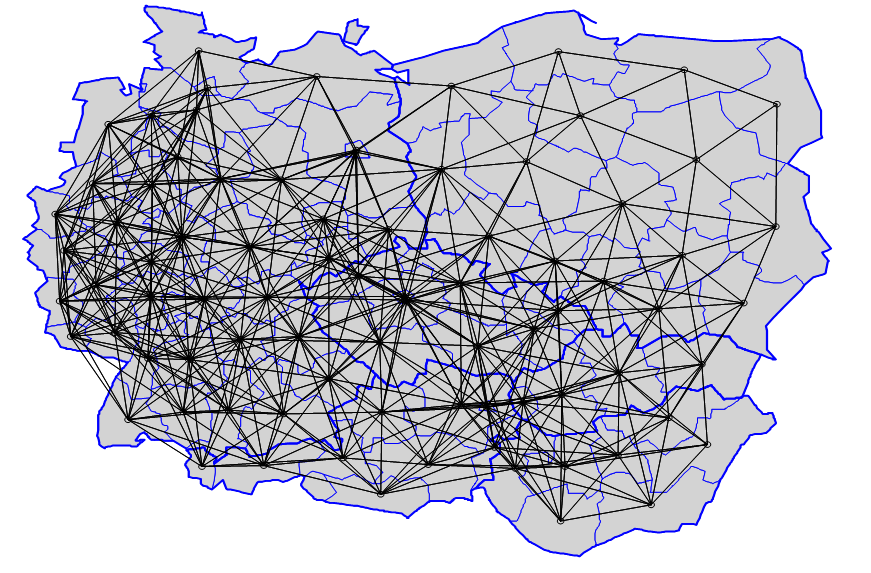
\includegraphics[width=.7\textwidth]{IMG/sp_neigb.PNG}
	\caption{Plot for distance-based neighbours (NUTS2), maximum neighbour distance threshold at 250 km}
\end{figure}
\end{frame}
%---------------------------------------------------------------------
\begin{frame}{Definice sousedících oblastí (Neighbours)}
\textbf{K-k-nejbližších sousedů(KNN)} \\
Za sousedící oblasti označíme předem stanovený počet k okolních oblastí, které jsou geograficky nejblíže. 
\begin{itemize}
	\item Řeší problémy s nestejnoměrnou geografickou hustotou (k sousedů zaručeno pro každou jednotku).
	\item Metoda obvykle vede k \textbf{asymetrickým prostorovým maticím} – obtížná interpretace sousednosti. $\dots$  existují jednoduché transformační algoritmy. 
	
	\item Příklad pro $k = 3$   (sousední oblasti vyobrazeny jen pro dvě jednotky):
	\begin{figure}
		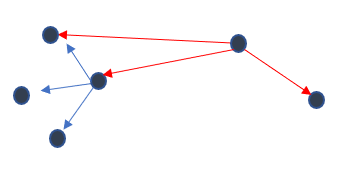
\includegraphics[width=.2\textwidth]{IMG/sp_neigb2.PNG}
	\end{figure}
\end{itemize}
\end{frame}
%---------------------------------------------------------------------
\section{Prostorové matice}
\begin{frame}{Prostorová matice – spatial matrix ($\bm{S}$)}
$$
\bm{S} = \begin{bmatrix}
0 & 1 & 1 & 1 \\
1 & 0 & 1 & 0 \\
1 & 1 & 0 & 1 \\
1 & 0 & 1 & 0
\end{bmatrix}\quad \text{příklad prostorové matice, počet jednotek: 4}$$
$$s_{ij}=
	\begin{cases}
	1, & \text{pokud jsou jednotky $i$ a $j$ sousedé.}\\
	1, & \text{nejde o sousedící jednotky}
	\end{cases}$$
\begin{itemize}
	\item Nuly na diagonále – jednotka není sama sobě sousedem.
	\item Interpetace prostorové matice: 
	\begin{itemize}
		\item 1. řádek (jednotka 1 sousedí s jednotkami 2,3,4
		\item 2. řádek jedntoka 2 sousedí s jednotkami 1,3 - ale nesousedí s jednotkou 4
		\item $\dots$ matice $\bm{S}$ je symetrická
	\end{itemize}
\end{itemize}
\end{frame}
%---------------------------------------------------------------------
\begin{frame}{Matice vah – weight matrix ($\bm{W}$)}
\vspace{-0.5cm}
$$
\bm{S} = \begin{bmatrix}
0 & 1 & 1 & 1 \\
1 & 0 & 1 & 0 \\
1 & 1 & 0 & 1 \\
1 & 0 & 1 & 0
\end{bmatrix}\rightarrow 
\bm{W}=
\begin{bmatrix}
0 & \tfrac{1}{3} & \tfrac{1}{3} & \tfrac{1}{3} \\[2pt]
\tfrac{1}{2} & 0 & \tfrac{1}{2} & 0 \\[2pt]
\tfrac{1}{3} & \tfrac{1}{3} & 0 & \tfrac{1}{3} \\[2pt]
\tfrac{1}{2} & 0 & \tfrac{1}{2} & 0
\end{bmatrix}
$$
\begin{itemize}
	\item Obvykle provedeme jednoduchou standardizaci $\bm{W}$ po řádcích: 
	$$ w_{ij} = \frac{s_{ij}}{\sum^n_{j=1} s_{ij}}$$
	$n$ - počet prostorových jednotek
	\item Nevhodné pro oblasti s heterogenní hustotou (velký vliv u oblastí s málo sousedy). 
	\item Binární indikátory $s_{ij}$ lze před standardizací zobecnit - například, místo binárních indikátorů využijeme předpoklad, že síla prostorové závislosti klesá se vzdáleností mezi jednotkami (lineárně, kvadraticky, atd.). Validita použitého prioru následně ovlivní přesnost/platnost informací, získaných prostorovou regresí.
\end{itemize}
\end{frame}
%---------------------------------------------------------------------
\begin{frame}{Matice vah – weight matrix ($\bm{W}$)}
$$
\bm{W}=
\begin{bmatrix}
0 & \tfrac{1}{3} & \tfrac{1}{3} & \tfrac{1}{3} \\[2pt]
\tfrac{1}{2} & 0 & \tfrac{1}{2} & 0 \\[2pt]
\tfrac{1}{3} & \tfrac{1}{3} & 0 & \tfrac{1}{3} \\[2pt]
\tfrac{1}{2} & 0 & \tfrac{1}{2} & 0
\end{bmatrix}
$$
\begin{itemize}
	\item Každý řádek matice $\bm{W}$ "tvoří" očekávanou hodnotu sledované proměnné - např. $y_i$ - na základě váženého průměru hodnot sousedních jednotek. Například:
	\begin{align*}
	\hat{y}_1 & =  \tfrac{1}{3} y_2 + \tfrac{1}{3} y_3 + \tfrac{1}{3} y_4 \\
	\dots \\
	\hat{y}_4 & = \tfrac{1}{2} y_1  + \tfrac{1}{3} y_3 
	\end{align*}
	\item Pozorované hodnoty proměnných u prostorových jednotek lze využít pro predikci příslušných hodnot u sousedících jednotek.
\end{itemize}
\end{frame}
%---------------------------------------------------------------------
\section{Moran's I, Geary's C}
\begin{frame}{Moran's $I$}
Nejčastěji uváděný a používaný test prostorové nezávislosti
$$I(x)_t = \big( \frac{n}{s}\big) \bm{x}^T_t \bm{W} \bm{x}_t (\bm{x}_t^T\bm{x}_t)^{-1}$$
kde $\bm{x}_t$ je vektor $n$ prostorových pozorování (jednotek) proměnné $x$ v čase $t$. 
$$S = \sum_{i=1}^n\sum_{j=1}^n w_{ij}$$
$S$ je standardizační faktor – součet všech členů matice $\bm{W}$. \\
$H_0 :$ absence prostorové závislosti, prostorová náhodnost (spatial randomness) \\
Očekávaná hodnota statistiky  $I(x)_t$ při platnosti $H_0 : \frac{-1}{(n-1)} $.\\
Pomocí $Var(I(x)_t)$ vypočteme $z$-poměr a testujeme statistickou významnost: zda jsou si sousedící jednotky více podobné, než by odpovídalo platné $H_0$. \\
Znaménko Moran's $I$ statistiky rozlišuje mezi pozitivní a negativní prostorovou autokorelací.
\end{frame}
%---------------------------------------------------------------------
\begin{frame}{Geary's $C$}
Geary's C je definován jako:
$$C = \frac{(N-1)\sum_i \sum_j w_{ij} (X_i - X_j)^2}{2W\sum_i (X_i -\bar{X})^2}$$
kde $N$ je počet prostorových jednotek; $X$ zkoumaná proměnná, $\bar{X}$ je průměrná hodnota, $w_{ij}$ jsou prvky matice vah a $W$ je součet všech prvků $w_{ij}$ . 
\begin{itemize}
	\item Geary's $C$ nabývá hodnotu mezi 0 a 2. 1 představuje prostorovou nezávislost. Hodnoty nižší než 1 znamenají pozitivní prostorovou autokorelaci, narůstající směrem k nule. Hodnoty vyšší než 1, indikují negativní prostorovou autokorelaci.
	\item Geary's $C$ je inverzně spjat se statistikou Moran's $I$. Zatímco Moran's $I$ popisuje celkovou prostorovou autokorelaci, Geary's $C$ je více citlivý na lokální vlivy.
\end{itemize}
\end{frame}
%---------------------------------------------------------------------
\section{Základní modely prostorové regrese}
\begin{frame}{Základní modely prostorové regrese}
\begin{figure}
	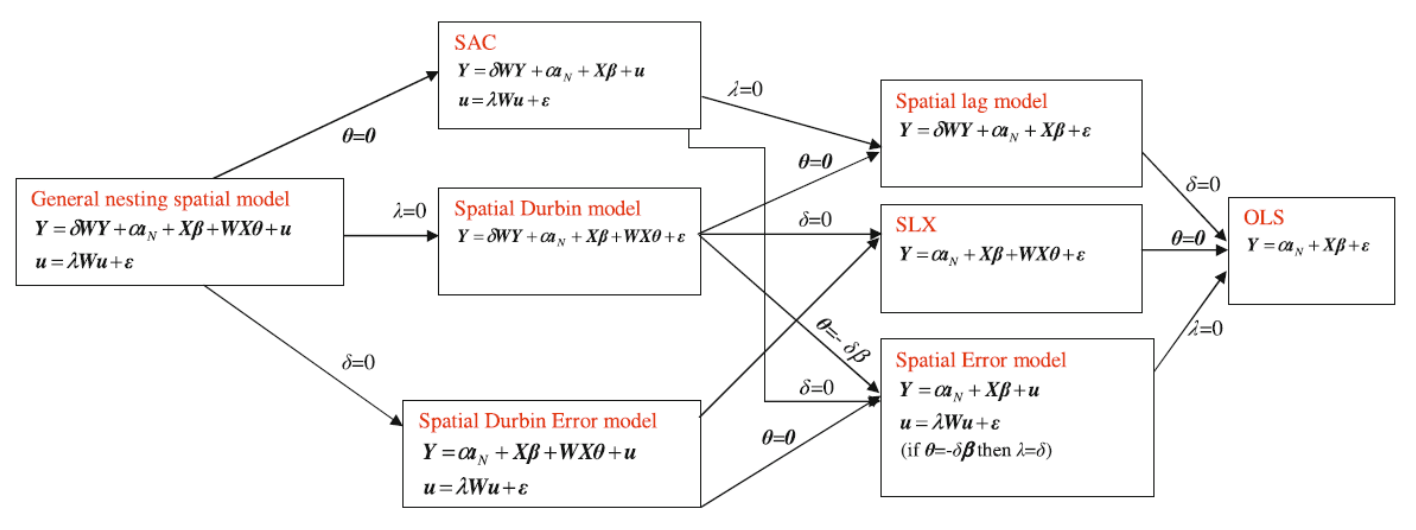
\includegraphics[width=.9\textwidth]{IMG/sp_reg.PNG}
	\caption{The rleationship betwee different spatial dependence models for cross-section data (source Halleck Vega and Elhorst 2012)}
\end{figure}
\end{frame}
%---------------------------------------------------------------------
\begin{frame}{Základní modely prostorové regrese}
\begin{itemize}
	\item \textbf{Prostorová autokorelace závislé proměnné}
	$$\bm{y}_t = \rho \bm{W}\bm{y}_t + \dots$$
	$\bm{Wy}_t$ popisuje prostorovou interakci mezi endogenními proměnnými modelu
	$\textit{SpatialLag}(y_{it}) = \bm{w}^T_i \bm{y}_t$, kde je $ \bm{w}^T_i$ řádek matice $\bm{W}$, $\bm{y}_t$ jsou pozorování $y$ v čase $t$.\\
	$\rho$ je koeficient prostorové autokorelace závislé proměnné (skalár); obvykle $\rho \in (-1,1)$.
	\item \textbf{Prostorová autokorelace regresorů}
	$$\bm{y}_t = \dots + \bm{X}_t \bm{\beta} + \bm{W}\bm{X}_t \bm{\theta} + \dots$$
	$\bm{X}$ je obvyklá matice regresorů, $\bm{WX}$ popisuje exogenní prostorové interakce mezi nezávislými proměnnými, $\bm{\beta}$ a $\bm{\theta}$ jsou vektory ($k\times 1$) neznámých parametrů, které se snažíme odhadnout.
\end{itemize}
\end{frame}
%---------------------------------------------------------------------
\begin{frame}{Základní modely prostorové regrese}
\begin{itemize}
	\item \textbf{Prostorová autokorelace náhodné složky} 
	$$\bm{u}_t = \lambda \bm{Wu}_t + \bm{\epsilon}_t$$
	 $\bm{Wu}_t$ popisuje prostorovou interakci mezi náhodnými složkami prostorových jednotek \\
	 $\lambda$ je koeficient prostorové autokorelace náhodné složky, resp. vynechaných prostorově  závislých vysvětlujících proměnných (skalár) \\
	 $\bm{\epsilon}_t$ vektor skutečných náhodných složek – prostorově nezávislá část náhodných složek.
	\item \textbf{Volba modelu se zahrnutím prostorové autokorelace} \\
		Konkrétní typ modelu volíme pomocí omezujících předpokladů: položíme $\rho,\theta$ nebo $\lambda$ rovné nule.
	Omezující předpoklady lze testovat. 
\end{itemize}
\end{frame}
%---------------------------------------------------------------------
\begin{frame}{Základní modely prostorové regrese}
\textbf{Spatial lag model}
\begin{itemize}
	\item Zajímá-li nás prostorová interakce mezi pozorovanými hodnotami závislé proměnné. Prostorovou závislost (strukturu) zde předpokládáme pouze u endogenní proměnné modelu. Model, resp. jeho redukovaná forma, mají tvar: 
	\begin{align*}
	\bm{y}_t & = \rho \bm{Wy}_t + \bm{X}_t\bm{\beta}+ \bm{u}_t\\
	(\bm{I} - \rho \bm{W}) \bm{y}_t & = \bm{X}_t \bm{\beta} + \bm{u}_t
	\end{align*}
	\item Koeficienty $\rho$ i $\bm{\beta}$ jsou odhadnuty metodou maximální věrohodnosti (MLE). Koeficienty  $\bm{\beta}$  pomáhají vysvětlit tu část variability $\bm{y}$, která není vysvětlena prostorově.	
\end{itemize}
\end{frame}
%---------------------------------------------------------------------
\begin{frame}{Základní modely prostorové regrese}
\textbf{Spatial Durbin model}
\begin{itemize}
	\item Vznikne rozšířením specifikace Spatial lag model o prostorové interakce mezi regresory: 
		\begin{align*}
		\bm{y}_t & = \rho \bm{Wy}_t + \bm{X}_t\bm{\beta}+ \bm{Wy}_t\bm{X}_t\bm{\theta} +  \bm{u}_t\\
		(\bm{I} - \rho \bm{W}) \bm{y}_t & = \bm{X}_t \bm{\beta} + \bm{Wy}_t\bm{X}_t\bm{\theta}+ \bm{u}_t
		\end{align*}
\end{itemize}
\end{frame}
%---------------------------------------------------------------------
\begin{frame}{Základní modely prostorové regrese}
\textbf{Spatial error model}
	\begin{align*}
	\bm{y}_t & =   \bm{X}_t\bm{\beta}+  \bm{u}_t, \qquad \bm{u}_t = \lambda  \bm{Wu}_t + \bm{\epsilon}_t\\
	\bm{y}_t & = \bm{X}_t\bm{\beta}+ \lambda\bm{Wy}_t\bm{u}_t+  \bm{\epsilon}_t\\
	(\bm{I} - \lambda \bm{W}) \bm{y}_t & = (\bm{I} - \lambda \bm{W}) \bm{X}_t \bm{\beta} + \bm{\epsilon}_t
	\end{align*}
\begin{itemize}

	\item I v případě, kdy se nezajímáme o prostorové interakce mezi pozorovanými proměnnými, můžeme zlepšit vlastnosti odhadu pomocí prostorově závislých chyb.
	\item Interakce v rámci náhodné složky nevyžadují teoretické zdůvodnění interakčního procesu, předpokládáme existenci prostorově závislých proměnných, nezahrnutých do modelu
\end{itemize}
\end{frame}
%---------------------------------------------------------------------
\begin{frame}{Prostorové modely:  stacionarita/stabilita}
\textbf{Stacionarita}
\begin{itemize}
\item Neformálně: pro každou oblast je počet sousedících oblastí omezený (malý)
\item Řádkové (a sloupcové) součty matice $\bm{S}$ jsou konečné a omezené, i když počet uvažovaných prostorových jednotek $n$ roste neomezeně.
\item Korelace mezi dvěma prostorovými jednotkami konverguje k nule s rostoucí vzdáleností mezi těmito jednotkami.
\item Formální podmínky stacionarity (pro $\rho, \lambda$ a $\bm{W}$ ) viz \href{https://www.google.cz/url?sa=t&rct=j&q=&esrc=s&source=web&cd=1&cad=rja&uact=8&ved=0ahUKEwjjwvLCk8bLAhXEvXIKHWSHBxsQFgggMAA&url=http://www.springer.com/cda/content/document/cda_downloaddocument/9783642403392-c2.pdf?SGWID\%3D0-0-45-1432965-p175381976&usg=AFQjCNGpme8ofJQzd46BCJVsUEio6oKIzQ&sig2=LlarV9wYhELGcTPiqzfRgg}{Elhorst (2014)}.
\end{itemize}
\end{frame}
%---------------------------------------------------------------------
\begin{frame}{Prostorové modely:  stacionarita/stabilita}
\textbf{Stabilita odhadů}
\begin{itemize}
	\item Matice $\bm{S}$, resp. matice $\bm{W}$ není odhadována, musíme ji stanovit předem. Odhadnuté koeficienty $\bm{\beta}$, resp. $\bm{\theta}$ závisejí na zvolené matici $\bm{W}$.
	\item "Řešení": regresní modely odhadujeme opakovaně, pokaždé s trochu jinak definovanou maticí $\bm{W}$ a porovnáváme vlastnosti jednotlivých odhadů.
    \item Tento postup zaručuje pouze lokální optimum (určíme nejlepší z porovnávaných modelů podle zvoleného kritéria), nikoliv globální optimum.
	\end{itemize}
\end{frame}
%---------------------------------------------------------------------
\section{Přímé a nepřímé efekty (Spill-overs)}
\begin{frame}{Přímé a nepřímé efekty (Spill-overs)}
\begin{itemize}
	\item $(\bm{I} - \rho \bm{W}) \bm{y}_t = \bm{X}_t \bm{\beta} + \bm{W}\bm{X}_t\bm{\theta} + \alpha \bm{\iota} +\bm{u}_t$ \quad $ \alpha \bm{\iota}$ je vektor úroňových konstant
	\item $\bm{y}_t = (\bm{I} - \rho \bm{W})^{-1} (\bm{X}_t\bm{\beta} + \bm{W}\bm{X}_t \bm{\theta})+ \bm{R}_t$ \quad 
	$\bm{R}_t$ obsahuje náhodnou složku i intercept 
\end{itemize}
Derivaci $E(\bm{y}_t)$ podle $k$-té vysvětlující proměnné $\bm{x}_{kt}$ lze zapsat jako:\\(časový index $t$ pro jednuduchost vynecháme)

\begin{align*} \bigg[\frac{\partial E(\bm{y})}{\partial \bm{x}_{1,k}} \dots \frac{\partial E(\bm{y})}{\partial \bm{x}_{N,k}}\bigg] & =
\begin{bmatrix}
\frac{\partial E(y_1)}{\partial \bm{x}_{1,k}} & \dots & \frac{\partial E(y_1)}{\partial \bm{x}_{N,k}} \\
\vdots & \ddots & \vdots \\
\frac{\partial E(y_N)}{\partial \bm{x}_{1,k}} & \dots & \frac{\partial E(y_N)}{\partial \bm{x}_{N,k}}
\end{bmatrix} = \\
& = (\bm{I} - \rho \bm{W})^{-1} 
\begin{bmatrix}
\beta_k & w_{12}\theta_k & \dots & w_{1N}\theta_k \\
w_{21}\theta_K & \beta_k & \dots & w_{2N}\theta_k \\
\vdots & \ddots & \ddots & \vdots \\
w_{N1}\theta_k & w_{N2}\theta_k & \dots & \beta_k 
\end{bmatrix}
\end{align*}
\end{frame}
%---------------------------------------------------------------------
\begin{frame}{Přímé a nepřímé efekty (Spill-overs)}
$$ \bigg[\frac{\partial E(\bm{y})}{\partial \bm{x}_{1,k}} \dots \frac{\partial E(\bm{y})}{\partial \bm{x}_{N,k}}\bigg] =
 (\bm{I} - \rho \bm{W})^{-1} 
\begin{bmatrix}
\beta_k & w_{12}\theta_k & \dots & w_{1N}\theta_k \\
w_{21}\theta_K & \beta_k & \dots & w_{2N}\theta_k \\
\vdots & \ddots & \ddots & \vdots \\
w_{N1}\theta_k & w_{N2}\theta_k & \dots & \beta_k 
\end{bmatrix}
$$
%---------------------------------------------------------------------
\begin{itemize}
	\item Změním-li hodnotu vysvětlující proměnné $x_k$ u $i$-té prostorové jednotky (změna $x_{ik}$), dojde ke změně očekávané hodnoty $y_i$ - \textbf{přímý efekt} a zároveň dojde ke změně očekávané hodnoty $y$ u dalších prostorových jednotek – \textbf{nepřímý efekt}. 
	\item Diagonální prvky matice (RHS) představují přímé efekty, prvky mimo diagonálu jsou nepřímé efekty
\end{itemize}

\end{frame}
%---------------------------------------------------------------------
\begin{frame}{Přímé a nepřímé efekty (Spill-overs)}
$$ \bigg[\frac{\partial E(\bm{y})}{\partial \bm{x}_{1,k}} \dots \frac{\partial E(\bm{y})}{\partial \bm{x}_{N,k}}\bigg] =
(\bm{I} - \rho \bm{W})^{-1} 
\begin{bmatrix}
\beta_k & w_{12}\theta_k & \dots & w_{1N}\theta_k \\
w_{21}\theta_K & \beta_k & \dots & w_{2N}\theta_k \\
\vdots & \ddots & \ddots & \vdots \\
w_{N1}\theta_k & w_{N2}\theta_k & \dots & \beta_k 
\end{bmatrix}
$$

\begin{itemize}
	\item Přímé a nepřímé efekty se liší pro jednotlivé prostorové jednotky ($i$).
	\begin{itemize}
	\item 	Přímé efekty se liší, protože diagonální prvky $(\bm{I} - \rho \bm{W})^{-1} $ jsou různé, pokud $\rho \neq 0$.
	\item Nepřímé efekty se liší, protože prvky mimo diagonálu matice $\bm{W}$, resp. $(\bm{I} - \rho \bm{W})^{-1}$ jsou různé, pokud $\rho \neq 0$ a/nebo $\theta_k \neq 0$
\end{itemize}
	$$ (\bm{I} - \rho \bm{W})^{-1} = \bm{I} + \rho\bm{W} + \rho^2\bm{W}^2 + \rho^3\bm{W}^3 + \dots$$

	\item Diagonální prvky matice (RHS) představují přímé efekty, prvky mimo diagonálu jsou nepřímé efekty
\end{itemize}
\end{frame}
%---------------------------------------------------------------------
\begin{frame}{Přímé a nepřímé efekty (Spill-overs)}
$$ \bigg[\frac{\partial E(\bm{y})}{\partial \bm{x}_{1,k}} \dots \frac{\partial E(\bm{y})}{\partial \bm{x}_{N,k}}\bigg] =
(\bm{I} - \rho \bm{W})^{-1} 
\begin{bmatrix}
\beta_k & w_{12}\theta_k & \dots & w_{1N}\theta_k \\
w_{21}\theta_K & \beta_k & \dots & w_{2N}\theta_k \\
\vdots & \ddots & \ddots & \vdots \\
w_{N1}\theta_k & w_{N2}\theta_k & \dots & \beta_k 
\end{bmatrix}
$$
%---------------------------------------------------------------------
\begin{itemize}
\item \textbf{Interpretace odhadnutého prostorového regresního modelu – vždy na základě přímých a nepřímých efektů}. 
\item Koeficient $\beta_k$ nepopisuje chování závislé proměnné $y_i$ při změně $x_{ik}$ "správně".
\item Statistickou významnost přímých efektů můžeme testovat viz \href{https://www.google.cz/url?sa=t&rct=j&q=&esrc=s&source=web&cd=1&cad=rja&uact=8&ved=0ahUKEwjjwvLCk8bLAhXEvXIKHWSHBxsQFgggMAA&url=http://www.springer.com/cda/content/document/cda_downloaddocument/9783642403392-c2.pdf?SGWID\%3D0-0-45-1432965-p175381976&usg=AFQjCNGpme8ofJQzd46BCJVsUEio6oKIzQ&sig2=LlarV9wYhELGcTPiqzfRgg}{Elhorst (2014)}.	
\end{itemize}
\end{frame}
%---------------------------------------------------------------------
\begin{frame}{Přímé a nepřímé efekty (Spill-overs)}
\begin{itemize}
	\item Ukázkový výstup odhadu přímých a nepřímých efektů (LeSage/Pace, 2009):
	$$\bm{y} = (\bm{I} - \rho \bm{W})^{-1} \bm{X}\bm{\beta} + (\bm{I} - \rho \bm{W})^{-1} \bm{\epsilon}$$
	$\dots$ jednoduchá regrese $y$ na $x$, použita prostorová regrese: \\
	Spatial lag model.
	
	\end{itemize}
\begin{table}[]
\centering
\caption{Spatial partitioning of direct, indirect and total   impacts}
\begin{tabular}{llll}
&         &          &             \\
                                                                                                       & Mean    & Std. dev & t-statistic \\
Direct effect                                                                                          & 0.586   & 0.0148   & 39.6106     \\
Indirect effect                                                                                        & 1.08414 & 0.0587   & 18.4745     \\
Total effect                                                                                           & 1.67    & 0.0735   & 22.7302    
\end{tabular}
\end{table}
\end{frame}
%---------------------------------------------------------------------
\begin{frame}{Přímé a nepřímé efekty (Spill-overs)}

$$ \bigg[\frac{\partial E(\bm{y})}{\partial \bm{x}_{1,k}} \dots \frac{\partial E(\bm{y})}{\partial \bm{x}_{N,k}}\bigg] =
(\bm{I} - \rho \bm{W})^{-1} 
\begin{bmatrix}
\beta_k & w_{12}\theta_k & \dots & w_{1N}\theta_k \\
w_{21}\theta_K & \beta_k & \dots & w_{2N}\theta_k \\
\vdots & \ddots & \ddots & \vdots \\
w_{N1}\theta_k & w_{N2}\theta_k & \dots & \beta_k 
\end{bmatrix}
$$
\begin{itemize}
	\item \textbf{Nevýhody, omezení modelů založených na prostorové závislosti:}
	\item Poměr přímého a nepřímého efektu nezávisí na $\beta_k$ - je dán pouze na základě matice $\bm{W}$ a hodnoty $\rho$. 
	\item Tento poměr je stejný pro všechny vysvětlující proměnné (resp. příslušné přímé a nepřímé efekty).
\end{itemize}

\end{frame}
%---------------------------------------------------------------------
\section{Identifikace hotspotů a coldspotů}
\begin{frame}{Identifikace "hotspotů" a "coldspotů"}
\begin{itemize}
	\item \textbf{Getis-Ord $G^\ast_i$}
	$$ G^\ast_i = \frac{\sum_{j=1}^n w_{i,j} x_j - \bar{X} \sum_{j=1}^n w_{i,j}}{S \quad\sqrt[]{\frac{[n\sum_{j=1}^n w^2_{i,j}-(\sum_{j=1}^n w_{i,j})^2]}{n-1}}}$$
	$$ \bar{X} = \frac{\sum_{j=1}^n x_j}{n}, \quad S = \sqrt[]{\frac{\sum_{j=1}^n x^2_j}{n}-(\bar{X})^2} $$
	\item $x_j$ je hodnota sledované proměnné v $j$-té jednotce, $w_{i,j}$ jsou prvky matice $\bm{W}$,  $n$ je počet prostorových jednotek.
	\item $G^\ast_i$ statistika se používá pouze pro kladnou prostorovou autokorelaci a umožňuje identifikovat prostorové shluky jednotek, které mají podobné hodnoty, jež jsou vysoké nebo nízké vůči průměrné pozorované hodnotě – hotspoty a coldspoty.\\(Getis – Ord 1992).
\end{itemize}
\end{frame}
%---------------------------------------------------------------------
\begin{frame}{Identifikace "hotspotů" a "coldspotů"}
\begin{figure}
	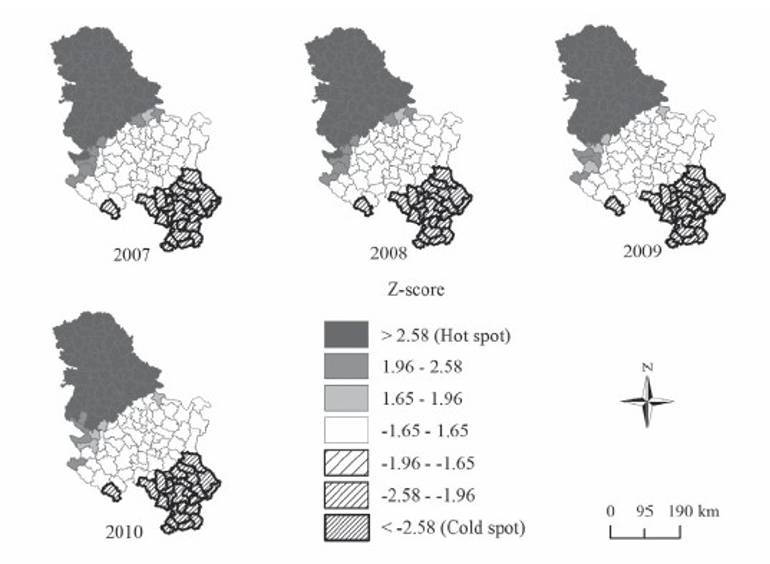
\includegraphics[width=.7\textwidth]{IMG/sp_coldspot.PNG}
	\caption{Spatial clusters (hot and cold spots) of the municipalities in Serbia by the level of average monthly net earning from 2001 to 2010 (at fix distance of 210 km)}
\end{figure}
\end{frame}
%---------------------------------------------------------------------
\begin{frame}{Identifikace "hotspotů" a "coldspotů"}
	$$ G^\ast_i = \frac{\sum_{j=1}^n w_{i,j} x_j - \bar{X} \sum_{j=1}^n w_{i,j}}{S \quad \sqrt[]{\frac{[n\sum_{j=1}^n w^2_{i,j}-(\sum_{j=1}^n w_{i,j})^2]}{n-1}}}$$
\begin{itemize}
	\item $ G^\ast_i$ je lokální statistika – spočtená pro každou prostorovou jednotku, jedná se o tzv. $z$-poměr ($z$-score).
	\item $ G^\ast_i$ popisuje statistickou významnost prostorového shlukování. Vysoká pozitivní hodnota $G^\ast_i$ indikuje koncentraci vysokých hodnot u sousedících prostorových jednotek (hotspot). Naopak, negativní hodnoty indikují výskyt tzv. coldspotu.
	\item Hodnoty blízké nule naznačují, že jednotka není součástí žádného prostorového shluku.
	
\end{itemize}
\end{frame}
%---------------------------------------------------------------------
\section{Prostorová regrese v R}
\begin{frame}{Prostorová regrese v R}
\begin{itemize}
	\item Knihovna \{spdep\} 
	\begin{itemize}
		\item Různé typy prostorových modelů
		\item Testy prostorové nezávislosti, identifikace prostorových shluků,$\dots$
	\end{itemize}
	\item	Knihovna \{splm\}
	\begin{itemize}
		\item Prostorová regrese na panelových datech
	\end{itemize}
	\item Knihovna \{ggplot2\} + další nutné knihovny
	\begin{itemize}
		\item Kartogramy (infomapy) / choropleth maps
	\end{itemize}
\end{itemize}
 \begin{figure}
 	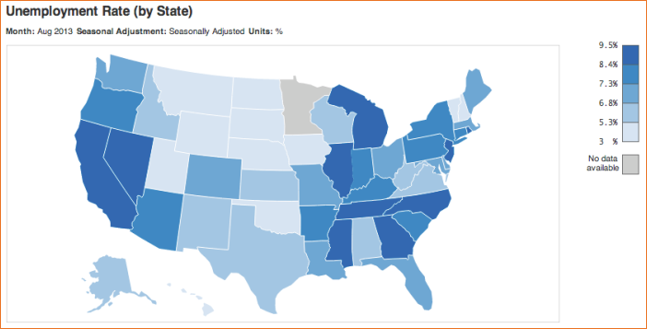
\includegraphics[width=.5\textwidth]{IMG/sp_unemp.PNG}
 \end{figure}

\end{frame}

%---------------------------------------------------------------------


\end{document}